
\section{Finding the meaning of Wikipedia Articles}
It is essential to know the meaning of the Wikipedia articles to be able to categorize them. 
Our assumption is that the meaning of Wikipedia articles can be found by looking at the categories leading to the article in the underlying category structure of Wikipedia. We base this assumption on the fact that all Wikipedia articles are placed under at least one category, and that the articles' categories should be representative for the article. This means that we need to find a representation for the underlying structure and a way of deciding the best way of reaching each article within this structure.
%One of the most common ways
%One way of finding the meaning of WIkipedia articles is by looking at Wikipedia's underlying structure since all Wikipedia articles are placed in categories. 

% One of the most commonly used strategies of finding the meaning of the articles is by looking at the 

\subsection{Representing the underlying structure}
Taking advantage of the underlying structure of Wikipedia requires a way of representing it. Each category has links to its subcategories, and links to the articles which are placed under the category (see figure \ref{fig:graphstructure}). Representing the structure could be split into two parts; one structure representing the underlying category structure (see figure \ref{fig:categorystructure}), and one structure representing the categories of each article (see figure \ref{fig:articlestructure}).  %representing the structure between categories, and representing the structure between categories and articles. 

\begin{figure}
\centering
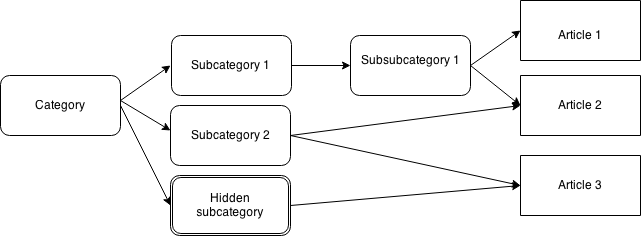
\includegraphics[width=\textwidth]{Chapters/Methods/graphstructure}
\caption{Simplified illustration of the underlying strcutre of Wikipedia.}
\label{fig:graphstructure}
\end{figure}

\subsubsection{Category graph}
A category graph is a way of representing the links between categories. This structure contains information about which subcategories can be reached from each category. Figure \ref{fig:categorystructure}) illustrates the category graph for representing the structure. The nodes in the graph (rectangles with rounded corners) represent categories, and the edges (arrows) represent the relationships between categories. The graph illustrated is a directed graph since each edge represents the relationship between the two categories (e.g. \emph{Subcategory 1} is subcategory of \emph{Category} since the arrow points from \emph{Category} to \emph{Subcategory 1}).

\begin{comment}


The graph has to contain directed edges, which means that a category is considered the subcategory of another if the category is 

can be created by representing categories as nodes and links as a 


Graph: nodes are categories and the edges are hyperlinks. 
--> nodes are categories and the edges are links between categories 


Such a graph is represented with all subcategories of a category listed under the category. The results of this is a structure like the illustration in figure \ref{fig:categorystructure}).
\end{comment}

%A category graph is a way of representing links between categories i.e., which categories can be reached from each category. The file containing all links between categories can be used to create such a graph. This is done by finding all subcategories of each category and remove all duplicate links. The results of this is a structure like the illustration in figure \ref{fig:categorystructure}).
\begin{figure}[h]
\centering
\begin{subfigure}[b]{0.4\textwidth}
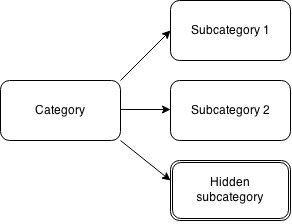
\includegraphics[width=\textwidth]{Chapters/Implementation/category-subcategories}
\caption{The structure where each category knows its subcategories}
\label{fig:categorystructure}
\end{subfigure}
\begin{subfigure}[b]{0.4\textwidth}
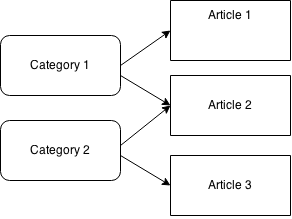
\includegraphics[width=\textwidth]{Chapters/Implementation/categories-articles}
\caption{The structure where each category know the title of its articles}
\label{fig:articlestructure}
\end{subfigure}
\caption[The representation of the Wikipedia structure]{Combined this is the structure needed to represent the Wikipedia's underlying category structure as a graph}
\end{figure}


\subsubsection{Article graph}
A different structure is desirable for representing articles and their most describing categories (the categories shown at the bottom of the article page in Wikipedia). The file containing all links between categories and their articles can be used to create a structure where each category knows its articles. Figure \ref{fig:articlestructure}) illustrates this structure. 

%It is desirable to remove articles whose titles are not relevant for our project. Numbers without context is an example of Wikipedia article titles that are difficult to determine the meaning since a number could have various meanings, including temperatures, grades or years. Hence, all article titles which only contains numbers could be disregarded. Wikipedia contains many such articles, and a total of 23 227 articles where found. This reduces the number of links betweeen articles and categories as shown in table  \ref{tab:withoutnumber}.

\begin{comment}
It is important that the category names are equal all places they occur. Wikipedia is written by volunteers from all over the worlds, and users might use different encoding depending on where they are from. Thus, both a cleaning process and a normalization process should be performed on all category names. The cleaning process is to make the category names look readable, while the normalization is a process where all words are made equal regardless of character encoding \cite[p.~26]{iirbook}.

The cleaning process includes converting all words to lowercase, replacing underscores with spaces and splitting up all titles containing the code for newline (\emph{\textbackslash n}). Newline is a way of representing how the articles should be sorted, figure \ref{fig:withnewline} is an example of an \texttt{INSERT} statement with newline in the title of the category, where the category should be sorted as if the title was \emph{ducks} as seen in figure \ref{fig:fictionalbirds}. Hence, the relevant part of the category title is the part after the newline, and this is the part that is considered further in the results. 


\begin{equation}\label{eq:removehiddencat}
a = 0
\end{equation}
\end{comment}

\subsubsection{Representing category and article names}
\emph{Id mapping} is a storage efficient way of representing category names and article titles because category names and article titles usually are longer than their representing ids. The id mapper is implemented by creating a counter that assigns a unique number to each category name or article title not already observed. 

\begin{comment}
The files containing the results becomes extremely large due to the size of the results. When writing all the results to file, the files becomes extremely large. All paths of all Wikipedia articles is more than 20 GB of compressed data. It is desirable to reduce the space needed for storing all results on the computer. The solution was to create an id mapping for each category name and article name. Id mapping gives all names a unique id, and instead of writing the full path of category names to the file, the full paths with category ids is written to file. 

The id mapping is implemented by creating a counter that assigns numbers to each category name or article name that is not found yet, i.e., a unique number represents each name. Figure \ref{fig:idmapping} shows an excerpt of the id mapping created for our purpose, where the id \emph{4600570} corresponds to the article about \emph{Ole-Johan Dahl}, which means that this id is used everywhere \emph{Ole-Johan Dahl} is used in paths. 

Id mapping is storage efficient because category names and article names usually are a  lot longer than their representing ids. 

Working with ids is also faster in many implementations concerning lookups in the program. This depends on the structure chosen for the programs, but when using dictionaries as done in our implementation, ids will perform faster than if using full names. An example of this can be seen in figure \ref{fig:id_lookup} where the time to find all categories from the category with id 177678 (corresponding to the category \emph{people}) is 0.955 minutes. Figure \ref{fig:fullname_lookup} shows the time needed to find the same paths for the category when using full names for categories and articles, which is found to be 1.559 minutes. Comparing the times shows that the time is a lot faster when using ids, which is important when many paths have to found.

The last reason to use ids instead of full names is that the full names may include characters useful for describing paths, for instance the characters "/" which is a common way of describing full paths. 

% Fordel 2: Kan bruke "/" in the text. 


\end{comment}